\documentclass{report}
\usepackage{ucs} 
\usepackage[utf8x]{inputenc} 	
\usepackage[czech]{babel}
\usepackage{pdfpages}
\usepackage{graphicx}
\usepackage{hyperref}
\usepackage{graphicx}
\usepackage{datetime}
\usepackage{titlesec}
\usepackage{interval}
\usepackage{multirow}
\usepackage{tikz-timing}
\usepackage{tikz}
\usepackage{listings}

\graphicspath{ {./Schematics/} }
\newcommand*\wildcard[2][5cm]{\vspace*{2cm}\parbox{#1}{\hrulefill\par#2}}  

\title{TuxMan - FPGA}
\titleformat{\paragraph}
\date{11/4/2019}
\author{Martin Přívozník}

\begin{document}
  \includepdf[page={1}]{Front-Page}
  \newpage
  \pagenumbering{gobble}

 \section*{Anotace (Resumé)}
 Tématem práce je návrh arkádové hry na RTL úrovni a její implementace na programovatelném hradlovém poli, tj. FPGA. Uživatelský vstup je zajištěn pomocí PS/2 klávesnice a výstup prostřednictvím VGA. K implementaci je použit jazyk VHDL.

\section*{Klíčová slova}
RTL, programovatelné hradlové pole, FPGA, PS/2, VGA, VHDL

 \section*{Summary}
 The topic of this thesis is designing an arcade game on an RTL level and its implementation on a programmable gate array, i.e. FPGA. User input is provided by PS/2 keyboard and output is shown using VGA. Language called VHDL is used for implementation.

\section*{Keywords}
RTL, programmable gate array, FPGA, PS/2, VGA, VHDL

 \newpage
\vspace*{\fill}

 \section*{Čestné prohlášení}
 Prohlašuji, že jsem předkládanou maturitní/ročníkovou práci vypracoval sám a uvedl jsem veškerou použitou literaturu a bibliografické citace.

\vspace{ 2cm}
  V Liberci dne \today
  \hspace{2cm}
  \wildcard{Martin Přívozník}

\newpage
\tableofcontents

\newpage
\pagenumbering{arabic}

\chapter*{Úvod}
\addcontentsline{toc}{section}{Úvod}

\chapter{Analýza}
Tato kapitola obsahuje stručný souhrn znalostí a informací potřebných pro následný návrh a implementaci. V sekci~\ref{sec:cislicovynavrh} je vysvětlen číslicový obvod a postup jeho návrhu. V sekci~\ref{sec:fpga} stručně vysvětluji programovatelné hradlové pole a dále vybranou vývojovou desku. Sekce~\ref{sec:rozhrani} se zabývá použitými komunikačními rozhraními, které zajišťují uživatelský vstup a výstup. Na závěr kapitoly, v sekci~\ref{sec:hrapacman} vysvětluji princip a funkčnost hry, jenž je vzorem pro můj návrh.

\section{Číslicový návrh}\label{sec:cislicovynavrh}
V této sekci se věnuji tomu, co je číslicový obvod a jak jej navrhnout jak ve schématu, tak v jazyce popisujícím hardware. V podsekci~\ref{sec:kombinacniobvody} rozeberu logické funkce, prostředky jejich popisu a realizace pomocí logických hradel. Podsekce~\ref{sec:sekvencniobvody}  je zaměřená na návrh sekvenčních obvodů a synchronních sekvenčních automatů (FSM), na což naváže podsekce~\ref{sec:synchronniaasynchronninavrh}, ve které vysvěluji princip hodinových domén a plně sekvenčního návrhu. V podsekci~\ref{sec:jazykvhdl} stručně ukážu, jak převést schéma číslicového obvodu do kódu v jazyce popisujícím hardware (Hardware Description Language, HDL), v mém případě do jazyka Very High Speed Integrated Circuit Hardware Description Language (VHDL).


\subsection{Kombinační obvody}\label{sec:kombinacniobvody}
\subsubsection{Booleovská funkce}
Booleovská funkce je funkce $N$ vstupů a $M$ výstupů nad množinou $\{0, 1\}$. V případě, kdy má funkce více jak jeden výstup, lze ji rozdělit na $M$ funkcí s jedním výstupem. Uvážíme-li Booleovu algebru, platí pro operace sčítání a násobení pravidla uvedená v tabulce~\ref{tab:pravidla}. 
\begin{table}
\centering
\begin{tabular}{ c c c } 
	$a+ b = b + a$ & $a*b = b*a$ & (komutativita) \\
	$a+(b+c) = (a+b) + c$ & $a*(b*c) = (a*b)*c$ & (asociativita) \\
	$a+(b*c) = (a+b) * (a+c)$ & $a*(b+c) = (a*b) + (a*c)$ & (distributivita) \\
	$a+0 = a$ & $a*1 = a$ & (neutralita 0 a 1) \\
	$a + \overline{a} = 1$ & $a * \overline{a} = 0$ & (vlastnosti negace) \\
\end{tabular}
    \caption{Axiomy a vztahy Booleovy algebry.\cite{boole1854investigation}}
    \label{tab:pravidla}
\end{table}
Operace se dvěma vstupními hodnotami nazýváme binární operace. Některé binární operace, přestože často používají stejná značení + a * jako v algebře reálných čísel, mají v Booleově algebře stejnou prioritu a jiný význam (žádná operace nemá přednost)~\cite{kubatova}. Pro logický součet a logický součin platí základní pravidla v tabulce~\ref{tab:pravidlaboolalgebry}.
\begin{table}
\centering
\begin{tabular}{ c c c } 
	de Morgan & $\overline{(a+b)} = \overline{a} * \overline{b}$ & $\overline{(a*b)} = \overline{a} + \overline{b}$ \\
	idempotence & $a + a = a$ & $a * a = a$ \\
\end{tabular}
    \caption{Základní pravidla Booleovy algebry.\cite{kubatova}}
    \label{tab:pravidlaboolalgebry}
\end{table}
Příkladem reprezentace Booleovské funkce je pravdivostní tabulka~\ref{tab:andtable}, kde $in_1$ a $in_2$ jsou vstupní hodnoty a $out$ je výstupní hodnota. 
\begin{table}
\centering
\begin{tabular}{ |c c|c| } 
   	\hline
	$in_1$ & $in_2$ & $out$ \\
	\hline
	$0$ & $0$ & $f(0,0)$ \\
	$0$ & $1$ & $f(0,1)$ \\
	$1$ & $0$ & $f(1,0)$ \\
	$1$ & $1$ & $f(1,1)$ \\
   	\hline
\end{tabular}
    \caption{Pravdivostní tabulka.}
    \label{tab:andtable}
\end{table}
Pravdivostní tabulka obsahuje vždy $N^2$ řádků, aby reprezentovala výstupní hodnotu pro všechny možné kombinace vstupních hodnot. Další možností je Booleovská formule~.\cite{kubatova}. K vyjádření formule a k popisu booleovské funkce používáme nejčastěji základní funkce uvedené v tabulce~\ref{tab:logickefunkce}
\begin{table}
\centering
\begin{tabular}{ |c|c|c| } 
   	\hline
	Název & Pravdivostní tabulka & Formule \\
   	\hline
	AND (logický součin) & \begin{tabular}{ |c c|c| } 
	   	\hline
		$in_1$ & $in_2$ & $out$ \\
	   	\hline
		$0$ & $0$ & $0$ \\
		$0$ & $1$ & $0$ \\
		$1$ & $0$ & $0$ \\
		$1$ & $1$ & $1$ \\
	   	\hline
	\end{tabular} & $out = in_1*in_2$ \\
   	\hline
	NAND (negovaný logický součin) & \begin{tabular}{ |c c|c| } 
	   	\hline
		$in_1$ & $in_2$ & $out$ \\
	   	\hline
		$0$ & $0$ & $1$ \\
		$0$ & $1$ & $1$ \\
		$1$ & $0$ & $1$ \\
		$1$ & $1$ & $0$ \\
	   	\hline
	\end{tabular} & $out = \overline{in_1*in_2}$ \\
	\hline
	OR (logický součet) & \begin{tabular}{ |c c|c| } 
	   	\hline
		$in_1$ & $in_2$ & $out$ \\
	   	\hline
		$0$ & $0$ & $0$ \\
		$0$ & $1$ & $1$ \\
		$1$ & $0$ & $1$ \\
		$1$ & $1$ & $1$ \\
	   	\hline
	\end{tabular} & $out = in_1+in_2$ \\
	\hline
	NOR (negovaný logický součet) & \begin{tabular}{ |c c|c| } 
	   	\hline
		$in_1$ & $in_2$ & $out$ \\
	   	\hline
		$0$ & $0$ & $1$ \\
		$0$ & $1$ & $0$ \\
		$1$ & $0$ & $0$ \\
		$1$ & $1$ & $0$ \\
	   	\hline
	\end{tabular} & $out = \overline{in_1+in_2}$ \\
	\hline
	NOT (logická negace) & \begin{tabular}{ |c|c| } 
	   	\hline
		$in_1$ & $out$ \\
	   	\hline
		$0$ & $1$ \\
		$1$ & $0$\\
	   	\hline
	\end{tabular} & $out = \overline{in_1}$ \\
	\hline
	BUFFER (opakovač) & \begin{tabular}{ |c|c| } 
	   	\hline
		$in_1$ & $out$ \\
	   	\hline
		$0$ & $0$ \\
		$1$ & $1$\\
	   	\hline
	\end{tabular} & $out = in_1$ \\
	\hline
	XOR (nonekvivalence) & \begin{tabular}{ |c c|c| } 
	   	\hline
		$in_1$ & $in_2$ & $out$ \\
	   	\hline
		$0$ & $0$ & $0$ \\
		$0$ & $1$ & $1$ \\
		$1$ & $0$ & $1$ \\
		$1$ & $1$ & $0$ \\
	   	\hline
	\end{tabular} & $out = in_1 \oplus in_2$ \\
	\hline
	XNOR (ekvivalence) & \begin{tabular}{ |c c|c| } 
	   	\hline
		$in_1$ & $in_2$ & $out$ \\
	   	\hline
		$0$ & $0$ & $1$ \\
		$0$ & $1$ & $0$ \\
		$1$ & $0$ & $0$ \\
		$1$ & $1$ & $1$ \\
	   	\hline
	\end{tabular} & $out =\overline{in_1 \oplus in_2}$ \\
   	\hline
\end{tabular}
    \caption{Tabulka nejpoužívanějších základních logických funkcí.}
    \label{tab:logickefunkce}
\end{table}
\subsubsection{Kombinační obvod}
Kombinační logický obvod, je takový obvod, ve kterém jsou výstupní hodnoty dány pouze aktuální kombinací vstupních proměnných. Neobsahuje žádnou paměť předchozích stavů. Jedinou vyjímkou je krátký časový interval, za který logický člen (AND, NAND, OR, NOR ...) vyhodnotí výstup na základě vstupních hodnot. Tento časový interval může být zanedbatelný v případě krátkých datových cest. V případě dlouhé datové cesty může být potřeba na tento časový interval brát zřetel a zvážit optimálnější řešení. \par
Platí, že u číslicových obvodů každá proměnná v operaci nabývá hodnotu jednoho tzv. bitu. Bit je základní jednotkou dat a může nabývat hodnot $0$, nebo $1$. Reprezentací číslicového obvodu je schéma číslicového obvodu, kde každá z funkcí je reprezentována tzv. schématickou značkou. Schématické značky mohou být různé, dokud z nich jasně vyplívá, jakou funkci zastupují. Schématické značky jsou propojené signály, které představují jednotlivé bity. Pro minimalizaci je možné několik signálů (bitů) zakreslit jediným konektorem, pokud je označený počtem bitů, které reprezentuje. Nejčastěji používané normy značení jsou evropská a americká. Příklady schéma\-tických značek pro nejpoužívanější logické funkce jsou uvedené v tabulce~\ref{tab:functionschemes}. 
\begin{table}
\centering
\begin{tabular}{ c c } 
	AND & \raisebox{-0.4\height}{\includegraphics[scale=0.6]{/Gates/AND.png}} \\
	NAND & \raisebox{-0.4\height}{\includegraphics[scale=0.6]{/Gates/NAND.png}} \\
	OR & \raisebox{-0.4\height}{\includegraphics[scale=0.6]{/Gates/OR.png}} \\
	NOR & \raisebox{-0.4\height}{\includegraphics[scale=0.6]{/Gates/NOR.png}} \\
	NOT & \raisebox{-0.4\height}{\includegraphics[scale=0.6]{/Gates/NOT.png}} \\
	BUFFER & \raisebox{-0.4\height}{\includegraphics[scale=0.6]{/Gates/BUFFER.png}} \\
	XOR & \raisebox{-0.4\height}{\includegraphics[scale=0.6]{/Gates/XOR.png}} \\
	XNOR & \raisebox{-0.4\height}{\includegraphics[scale=0.6]{/Gates/XNOR.png}} \\
\end{tabular}
    \caption{Schématické značky některých nejpouživanějších základních logických funkcí (americká norma ANSI).}
    \label{tab:functionschemes}
\end{table}
Pro usnad\-nění práce můžeme využívat logických bloků, které plní danou funkci. Opět platí, že ze značení logických bloků ve schématu musí plně vyplívat, jakou funkci zastupují. Logický blok, který má definovanou funkci může být použit schématu. Při návrhu číslicových obvodů využíváme hierarchie, kde jsou pro každý logický blok popsány vstupy i výstupy a v případě, kdy se nejedná o základní logické bloky, tak je popsána i funkce (formule, pravdivostní tabulka, nebo schéma bloku) a vhodně přiřazena ke schématu. Jedním ze základních logických bloků je poloviční sčítačka, viz obrázek~\ref{fig:halfadder}.
\begin{figure}
\centering
\includegraphics[width=0.9\columnwidth]{/LogicalBlocks/HalfAdder.png}
\caption{Schéma poloviční sčítačky a příklad jejího značení ve schématu.}
\label{fig:halfadder}
\end{figure}
 Poloviční sčítačka umí sečíst dvě jednobitová čísla a vygenerovat bit do vyššího řádu (carry) podle pravdivostní tabulky~\ref{tab:halfaddertab}.
\begin{table}
\centering
 \begin{tabular}{ |c c|c c| } 
   	\hline
	$A$ & $B$ & $C$ & $\sum$ \\
   	\hline
	$0$ & $0$ & $0$ & $0$ \\
	$0$ & $1$ & $0$ & $1$\\
	$1$ & $0$ & $0$ & $1$\\
	$1$ & $1$ & $1$ & $0$\\
   	\hline
\end{tabular}
	\caption{Pravdivostní tabulka poloviční sčítačky.}
	\label{tab:halfaddertab}
\end{table}
Zřetězením dvou polovičních sčítaček a přenesením pomocí funkce OR získáme poté kompletní sčítačku, viz obrázek~\ref{fig:fulladder}.\cite{kubatova}
\begin{figure}
\centering
\includegraphics[width=0.9\columnwidth]{/LogicalBlocks/FullAdder.pdf}
\caption{Schéma kompletní sčítačky a příklad jejího značení ve schématu.}
\label{fig:fulladder}
\end{figure}
Kompletní sčítačka umí sečíst jednobitová čísla, vygenerovat bit do vyššího řádu a přijmout bit z nižšího, sčítá tedy tři bity. Sčítá počet jedniček na vstupech. \par
Pro porovnávání dvou hodnot a vyhodnocení jejich nerovnosti používáme tzv. komparátor, viz obrázek~\ref{fig:comparator}. 
\begin{figure}
\centering
\includegraphics[width=0.9\columnwidth]{/LogicalBlocks/Comparator.pdf}
\caption{Schéma komparátoru a příklad jeho značení ve schématu.}
\label{fig:comparator}
\end{figure}
Dalším důležitým základním logickým blokem je multiplexor, viz obrázek~\ref{fig:mux}.
\begin{figure}
\centering
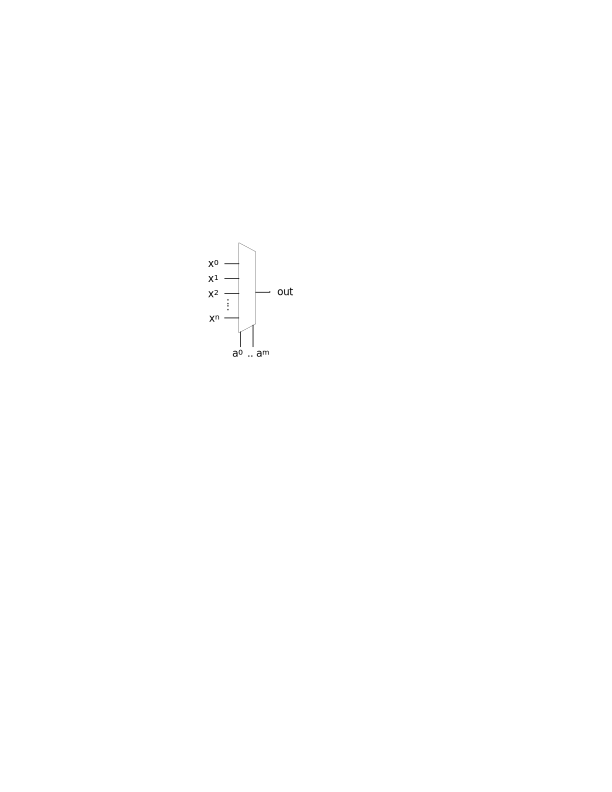
\includegraphics[width=0.6\columnwidth]{/LogicalBlocks/Mux.pdf}
\caption{Schématická značka multiplexoru.}
\label{fig:mux}
\end{figure}
Multiplexor na základě řídícího vstupu/řídících vstupů ($a$) přivádí na výstup ($out$) jeden ze vstupních signálů ($x$). \par
Číslicový obvod lze realizovat například z integrovaných obvodů, v nichž bývají hradla realizována z několika tranzistorů. Logické hodnoty představuje napětí přivedené na obvod. Logická $1$ bývá reprezentována  napětím kladným a logická $0$ napětím nulovým.

\subsection{Sekvenční obvody}\label{sec:sekvencniobvody}
\subsubsection{Sekvenční logický obvod}
Sekvenční logický obvod je takový obvod, ve kterém výstupní hodnoty nejsou dány pouze aktuální kombinací vstupních proměnných, ale zároveň předchozím stavem. Sekvenční obvod si tedy musí zapamatovat předchozí hodnoty pomocí paměti, která bývá realizována pomocí zpětné vazby~\cite{kubatova}. Sekvenční obvod se dělí na dvě části - kombinační a paměťovou, kde paměťová část je tvořena logickým obvodem, ve kterém bývá zavedena zpětná vazba a kombinační část bývá tvořena kombinačním obvodem. Obecné schéma sekvenčního obvodu je na obrázku~\ref{fig:seqcircuit}. \par
\begin{figure}
\centering
\includegraphics[width=0.9\columnwidth]{/LogicalBlocks/sqcircuit.pdf}
\caption{Huffmanův model sekvenčního obvodu.}
\label{fig:seqcircuit}
\end{figure}
Příkladem logického obvodu se zpětnou vazbou může být tzv. RS klopný obvod, viz obrázek~\ref{fig:rsko}.
\begin{figure}
\centering
\includegraphics[width=0.9\columnwidth]{/LogicalBlocks/RSKO.pdf}
\caption{Schéma RS klopného obvodu s využitím logických hradel NOR.}
\label{fig:rsko}
\end{figure}
RS klopný obvod překlápí mezi dvěma mezními hodnotami. Pravdivostní tabulka RS klopného obvodu se může dělit na tři části - zakázaný stav (ZS), překlápěcí část a paměť, viz tabulka~\ref{tab:rskotab}.
\begin{table}
\centering
 \begin{tabular}{ |c c|c c| } 
   	\hline
	$A$ & $B$ & $Q$ & $Q'$ \\
   	\hline
	$0$ & $0$ & \multicolumn{2}{c|}{Z.S.} \\
	$0$ & $1$ & $0$ & $1$\\
	$1$ & $0$ & $1$ & $0$\\
	$1$ & $1$ & \multicolumn{2}{c|}{Paměť}\\
   	\hline
\end{tabular}
	\caption{Pravdivostní tabulka RS klopného obvodu s využitím NOR.}
	\label{tab:rskotab}
\end{table}
Pokud se tedy změní vstupní hodnoty z $[0,1]$, nebo $[1,0]$ na $[1,1]$, na výstupu bude předchozí hodnota, dokud neproběhne další změna vstupních hodnot. Jedná se tedy o tzv. hladinový klopný obvod (angl. latch). Častěji využívaným klopným obvodem je tzv. D klopný obvod, viz obrázek~\ref{fig:dko}.
\begin{figure}
\centering
\includegraphics[width=0.9\columnwidth]{/LogicalBlocks/DKO.pdf}
\caption{Schéma D klopného obvodu.}
\label{fig:dko}
\end{figure}
Výhodou D klopného obvodu je fakt, že narozdíl od RS klopného obvodu nemá zakázaný stav, viz pravdivostní tabulka~\ref{tab:dkotab}.
\begin{table}
\centering
 \begin{tabular}{ |c c|c c| } 
   	\hline
	$T$ & $D$ & $Q$ & $Q'$ \\
   	\hline
	\texttiming{LH} & $x$ & $x$ & $\overline{x}$\\
	\multicolumn{2}{|c|}{Jinak} & \multicolumn{2}{|c|}{Paměť}\\
   	\hline
\end{tabular}
	\caption{Pravdivostní tabulka D klopného obvodu.}
	\label{tab:dkotab}
\end{table}
Signál $T$ u D klopného obvodu se dá považovat za tzv. povolovací signál. Při náběžné hraně na $T$  (změna stavu z logické $0$ na logickou $1$) se na výstup $Q$ zapíše aktuální hodnota na signálu $D$. V tomto případě se tedy jedná o hranový klopný obvod. Příklad značení D klopného obvodu je na obrázku~\ref{fig:dblock}.
\begin{figure}
\centering
\includegraphics[width=0.4\columnwidth]{/LogicalBlocks/DBlock.pdf}
\caption{Příklad značení D klopného obvodu ve schématu.}
\label{fig:dblock}
\end{figure}
Vstupní signál označený trojúhelníkem je signál T. Trojúhelník značí, že obvod mění výstupní hodnotu v reakci na náběžnou hranu. Tento vstup se jinak nazývá hodinovým vstupem. Pokud má číslicový obvod takový vstup jedná se o sekvenční obvod. V případě hladinového obvodu by ve značení byl místo trojúhelníku čtverec. \par
Hodnoty na signálech se dají popsat tzv. časovým diagramem. Časový diagram popisuje, jaké logické hodnoty nabývá daný signál v jaký čas. Příklad časového diagramu je na obrázku~\ref{fig:dkotd}.
\begin{figure}
\centering
\includegraphics[width=0.6\columnwidth]{/TimeDiagrams/DFlipFlop.pdf}
\caption{Časový diagram D klopného obvodu.}
\label{fig:dkotd}
\end{figure}
\par
Příkladem sekvenčního logického bloku je čítač. Čítač je takový sekvenční logický obvod, který uchovává v ,,paměti" informaci o tom, kolikrát zaznamenal změnu stavu (dle návrhu náběžnou, nebo sestupnou hrana) na hodinovém signálu. Příklad schématu čítače je na obrázku~\ref{fig:counter}.
\begin{figure}
\centering
\includegraphics[width=0.7\columnwidth]{/LogicalBlocks/Counter.pdf}
\caption{Příklad schématu dvoubitového čítače reagujícího na náběžnou hranu.}
\label{fig:counter}
\end{figure}
Může být ve schématu značen, jako na obrázku~\ref{fig:counterbox}.
\begin{figure}
\centering
\includegraphics[width=0.4\columnwidth]{/LogicalBlocks/Counterbox.pdf}
\caption{Příklad schématické značky dvoubitového čítače reagujícího na náběžnou hranu.}
\label{fig:counterbox}
\end{figure}
\subsubsection{Konečný stavový automat}
Konečný stavový automat (angl. Finite State Machine - FSM) M je šestice M=(Q, T, D, delta, lambda, q0), kde:
\begin{itemize}
  \item Q je konečná množina vnitřních stavů
  \item T je konečná množina vstupních symbolů (signálů)
  \item D je konečná množina výstupních symbolů (signálů)
  \item delta je zobrazení z Q x T do Q (stav x vstup do stav) nazývané přechodová funkce
  \item lambda je zobrazení z Q x T do D (Mealy, ze stavu a vstupu do výstupu) nebo Q do D (Moore, jen ze stavu do výstupu)
  \item q0 je počáteční stav
\end{itemize}
~\cite{jazykyapreklady} Má definované stavy, mezi kterými za daných podmínek přepíná a mění svůj výstup. FSM provádí vždy právě jeden přechod s každou náběžnou hranou hodin. Musí popisovat přechodovou funkci (podmínky pro změnu stavu a do kterého), výstupní funkci (jaký signál v danou chvíli udává na výstup) a dále musí mít definovaný počátečný stav. Příklad stavového diagramu FSM je na obrázku~\ref{fig:fsmexample}, kde $a, b, c$ jsou podmínky pro změnu stavu a $q1, q2, q3$ jsou stavy FSM. Počáteční stav je značen šipkou, která nevychází z žádného stavu, v tomto případě $q1$.
\begin{figure}
\begin{center}
\begin{tikzpicture}[scale=0.2]
\tikzstyle{every node}+=[inner sep=0pt]
\draw [black] (22.4,-28.4) circle (3);
\draw (22.4,-28.4) node {$q1$};
\draw [black] (39.9,-28.4) circle (3);
\draw (39.9,-28.4) node {$q2$};
\draw [black] (57.8,-28.4) circle (3);
\draw (57.8,-28.4) node {$q3$};
\draw [black] (25.4,-28.4) -- (36.9,-28.4);
\fill [black] (36.9,-28.4) -- (36.1,-27.9) -- (36.1,-28.9);
\draw (31.15,-27.9) node [above] {$a$};
\draw [black] (42.9,-28.4) -- (54.8,-28.4);
\fill [black] (54.8,-28.4) -- (54,-27.9) -- (54,-28.9);
\draw (48.85,-27.9) node [above] {$b$};
\draw [black] (55.587,-30.423) arc (-51.04855:-128.95145:24.636);
\fill [black] (24.61,-30.42) -- (24.92,-31.31) -- (25.55,-30.54);
\draw (40.1,-36.4) node [below] {$c$};
\draw [black] (15.5,-28.4) -- (19.4,-28.4);
\fill [black] (19.4,-28.4) -- (18.6,-27.9) -- (18.6,-28.9);
\end{tikzpicture}
\end{center}
\caption{Příklad stavového diagramu konečného stavového automatu.}
\label{fig:fsmexample}
\end{figure}
Rozeznáváme dva typy FSM na základě definičního oboru výstupní funkce~\cite{kubatova}. Prvním typem je typ Mealy (angl. často input-based), který mění svůj výstup na základě aktuálního stavu a změn na vstupních signálech. Druhý je typ Moore (angl. často state-based), jehož výstupní funkce je závislá pouze na aktuálním stavu (každý stav má definovaný výstup). Příkladem stavového diagramu čítače modulo 4 s povolujícím vstupem je obrázek~\ref{fig:counterfsm}
\begin{figure}
\begin{center}
\begin{tikzpicture}[scale=0.2]
\tikzstyle{every node}+=[inner sep=0pt]
\draw [black] (30.5,-22.2) circle (3);
\draw (30.5,-22.2) node {$q0/00$};
\draw [black] (53.2,-22.2) circle (3);
\draw (53.2,-22.2) node {$q1/01$};
\draw [black] (53.2,-41.8) circle (3);
\draw (53.2,-41.8) node {$q2/10$};
\draw [black] (30.5,-41.8) circle (3);
\draw (30.5,-41.8) node {$q3/11$};
\draw [black] (31.931,-19.572) arc (144.37918:35.62082:12.202);
\fill [black] (51.77,-19.57) -- (51.71,-18.63) -- (50.9,-19.21);
\draw (41.85,-13.98) node [above] {$CE\mbox{ }=\mbox{ }1$};
\draw [black] (55.984,-23.288) arc (60.10415:-60.10415:10.049);
\fill [black] (55.98,-40.71) -- (56.93,-40.75) -- (56.43,-39.88);
\draw (61.52,-32) node [right] {$CE\mbox{ }=\mbox{ }1$};
\draw [black] (19.5,-22.2) -- (27.5,-22.2);
\draw (19,-22.2) node [left] {$reset$};
\fill [black] (27.5,-22.2) -- (26.7,-21.7) -- (26.7,-22.7);
\draw [black] (51.63,-44.348) arc (-38.52063:-141.47937:12.5);
\fill [black] (32.07,-44.35) -- (32.18,-45.29) -- (32.96,-44.66);
\draw (41.85,-49.56) node [below] {$CE\mbox{ }=\mbox{ }1$};
\draw [black] (27.936,-40.262) arc (-129.04509:-230.95491:10.637);
\fill [black] (27.94,-23.74) -- (27,-23.85) -- (27.63,-24.63);
\draw (23.5,-32) node [left] {$CE\mbox{ }=\mbox{ }1$};
\draw [black] (33.287,-23.278) arc (96.59379:-191.40621:2.25);
\draw (38.43,-27.66) node [below] {$CE\mbox{ }=\mbox{ }0$};
\fill [black] (31.34,-25.07) -- (30.94,-25.92) -- (31.93,-25.81);
\draw [black] (54.87,-19.722) arc (173.74488:-114.25512:2.25);
\draw (59.72,-17.63) node [right] {$CE\mbox{ }=\mbox{ }0$};
\fill [black] (56.18,-22.02) -- (56.92,-22.6) -- (57.03,-21.61);
\draw [black] (55.834,-43.212) arc (89.53768:-198.46232:2.25);
\draw (60.47,-47.79) node [below] {$CE\mbox{ }=\mbox{ }0$};
\fill [black] (53.68,-44.75) -- (53.17,-45.55) -- (54.17,-45.55);
\draw [black] (29.391,-44.575) arc (5.94318:-282.05682:2.25);
\draw (24.94,-47.77) node [left] {$CE\mbox{ }=\mbox{ }0$};
\fill [black] (27.62,-42.61) -- (26.78,-42.19) -- (26.88,-43.19);
\end{tikzpicture}
\end{center}
\caption{Příklad stavového diagramu (typ Moore) čítače modulo 4 se vstupem count enable.}
\label{fig:counterfsm}
\end{figure}

\subsection{Synchronní návrh}\label{sec:synchronniaasynchronninavrh}
\subsubsection{Pravidla návrhu synchronního obvodu}
Synchronní obvod je takový obvod, ve kterém všechny sekvenční části obvodu mají na svůj hodinový vstup přivedený stejný signál, aby měnily svůj stav ve stejný čas. Tento signál můžeme nazývat společné hodiny. Společné hodiny mění svůj stav na dané frekvenci (nejčastěji dle krystalu v obvodu). Tuto část obvodu můžeme nazývat hodinová doména. Pro návrh synchronního návrhu platí několik pravidel, které je nutné dodržet pro správnost návrhu. Společné hodiny nesmí být hradlované (signál musí být přiveden přímo k hodinovým vstupům sekvenčních obvodů). V případě hradlování společných hodin může docházet k časovým rezervám v jednotlivých částech obvodu. Dále je nutné, aby obvod obsahoval synchronní reset. Po synchronním resetu obvodu změní stav celý obvod společně a nedojde k časovým nesrovnalostem.~\cite{hodinovedomeny} \par
Při návrhu se nemusí vždy pracovat pouze s jednou hodinovou doménou. V tomto případě je nutné společné hodiny synchronizovat specializovaným obvodem, který můžeme nazývat synchronizér. Synchronizér se může skládat z D klopných obvodů, které mají dané podmínky pro korektní funkci. Vstupní hodnota D klopného obvodu nesmí být změněna krátce před příchodem náběžné hrany na hodinovém vstupu (tj. předstih). Zároveň nesmí být změněna těsně po příchodu náběžné hrany na hodinovém vstupu (tj. přesah).~\cite{hodinovedomeny} V případě porušení těchto podmínek se může stát, že klopný obvod bude mít abnormálně zpožděnou, nebo kolísavou odezvu. Příklad synchronizéru je na obrázku\ref{fig:synchronizer}.
\begin{figure}
\centering
\includegraphics[width=0.9\columnwidth]{/LogicalBlocks/Synchronizer.pdf}
\caption{Příklad návrhu synchronizéru.}
\label{fig:synchronizer}
\end{figure}
\par
Datové signály jsou řízené řídícími signály synchronizéru. Protokol řídících signálů musí být navržen tak, aby se měnil vždy jen jeden. Řídící signál můžeme nazývat strobe. Úkolem tohoto protokolu je indikace, zda jsou data aktuální (tj. na signálu strobe bude logická $1$, dokud nezačne opět probíhat příchod nových dat).
\subsection{Jazyk VHDL}\label{sec:jazykvhdl}
\subsubsection{Charakteristika jazyka VHDL}
VHDL (VHSIC (Very-High-Speed Integrated Circuit, česky velmi rychlý integrovaný obvod) Hardware Description Language) je programovací jazyk sloužící pro popis hardware (tj. Hardware Description Language, zkr. HDL, česky jazyk popisující hardware). Používá se pro návrh digitálních integrovaných obvodů, např. u FPGA (Field of Programmable Gate Array, česky programovatelná hradlová pole). VHDL je silně typovaný jazyk a umožňuje popsat obvod na hradlové, RTL (Register Transfer Level, česky přenos na úrovni registrů) i algoritmické úrovni~\cite{vhdlI}.
\subsubsection{Datové typy}
VHDL je silně typovaný jazyk, při operacích je tedy nutné, aby se typy shodovaly. Jedny z důležitých základních datových typů jsou: , bit, integer, std\textunderscore logic a std\textunderscore logic\textunderscore vector, . 
\begin{itemize}
  \item Array - pole prvků jiného typu
  \item Bit - Výčtový typ ('0', '1')
  \item Integer - Celé číslo
  \item Std\textunderscore logic - Popis signálu ('U’,'X', '0',  ‘1', 'Z', 'W',  'L', 'H', '-')
  \item Std\textunderscore logic\textunderscore vector - Pole std\textunderscore logic
  \item Signed - Bitový vektor, který nepopisuje stav signálu, ale pouze číselnou hodnotu
  \item Unsigned - Signed, který může obsahovat pouze kladné hodnoty
\end{itemize}

\subsubsection{Základní konstrukce}
Konstrukce jazyka VHDL se dělí na několik částí. Jednou z nich je tzv. entita. Entita popisuje pouze rozhraní, nikoliv chování, nebo vnitřní strukturu návrhu. Obsahuje tedy definici vstupních a výstupních portů. Příklad návrhu entity multiplexoru se dvěma datovými vstupy $A, B$, jedním řídícím vstupem $SEL$ a výstupem $Y$:
\begin{lstlisting}[language=VHDL]
entity MULTIPLEXER is
port(   A, B, SEL 	: in bit;
	Y		: out bit
	);
end MULTIPLEXER;
\end{lstlisting}
Další částí je architektura. Architektura obsahuje chování a vnitřní strukturu entity. Architektura tedy musí být definována uvnitř entity a nelze, aby fungovala samostatně. Entita může obsahovat více architektur. Ta se poté dělí na dvě části. Deklarační a sekci paralelních příkazů. Deklarační část se nachází před klíčovým slovem begin a je vyhrazena pro deklaraci signálů, konstant, nebo typů. Součástí sekce paralelních příkazů může být instance koponent, behaviorální popis (tj. popis chování), nebo tzv. procesy a nachází se v tělě architektury (tj. část za klíčovým slovem begin). Příklad architektury výše uvedeného multiplexoru:
\begin{lstlisting}[language=VHDL]
architecture MUX_BODY of MULTIPLEXER is

signal SELNON, ASEL, BSEL : std_logic;

begin

SELNON <= not SEL;
ASEL <= A and SELNON;
BSEL <= B and SEL;
Y <= ASEL or BSEL;

end MUX_BODY;
\end{lstlisting}
Proměnná označená klíčovým slovem signal značí stejnojmenný signál v obvodu. Klíčové slovo $std\textunderscore logic$ říká, že se jedná o jednobitový signál. V případě vícebitového signálu by bylo využito klíčové slovo $std\textunderscore logic\textunderscore vector$. Signál si pamatuje svou hodnotu, dokud není změněna dalším přiřazením.~\cite{vhdlI} V části paralelních příkazů operátor $<=$ zastupuje operátor přiřazení. Hodnota z pravé strany je tedy po vyhodnocení logické operace přiřazena signálu na levé straně. Všechny logické operace v tomto případě jsou vyhodnocovány paralelně. Tato metoda se většinou využívá pro popis chování kombinačních obvodů. V případě popisu sekvenčního obvodu je nejčastěji využíván tzv. proces. Proces je součástí architektury a i přes to, že popisuje sekvenční obvod, tak běží souběžně. V sekvenčním popisu je možné krom operátorů přiřazení a logických operací využívat také podmínky, jako je např. $if$, nebo $case$. V případě psaní syntetizovatelného kódu proces obsahuje citlivostní seznam a opět popis chování. Citlivostní seznam je seznam signálů, na který sekvenční obvod reaguje (u sekvenčních obvodů hodinový vstup a synchronní reset). Příklad procesu, který popisuje D klopný obvod, kde $D$ je vstupní hodnota, $Q$ je výstupní, $clk$ jsou hodiny a $reset$ je synchronní reset:
\begin{lstlisting}[language=VHDL]
D_FLIP_FLOP : process (clk, reset)
begin
	if(clk'event and clk='1') then       
		if(reset = '1') then
			Q <= '0';
		else 
			Q <= D;
		end if;
	end if;
end process;
\end{lstlisting}
Pokud na hodinách obvod zaznamená náběžnou hranu a není aktivní synchronní reset, tak na signál $Q$ zapíše aktuální hodnotu na signálu $D$. \par
Celý obvod je možné popsat v rámci jedné entity, pro přehlednost je možné ale využívat componenty. Při návrhu většího obvodu je vhodné logicky oddělit části obvodů od sebe a vytvořit z nich entity, které je možné poté propojit v nadřazené entitě pomocí klíčového slova component a namapování vstupních a výstupních signálů jednotlivých entit pomocí příkazu port map. Při mapování je poté možné pouze přiřadit vstupní a výstupní signály k signálům v nadřazené entitě~\cite{vhdlI}.  
\subsubsection{Popis FSM}
Jazyk VHDL nezná pojem automatu a existuje mnoho způsobů, jak jej popsat ve VHDL. Často používaný popis a zároveň takový, který usnadní práci logické syntéze programu je metoda se třemi procesy. Prvním procesem je přechodová funkce a jedná se o kombinační proces, který na základě vstupních hodnot vyhodnocuje, jaký bude příští stav FSM. Vstupy přechodové funkce jsou stavy a vstupy FSM a jejím výstupem je příští stav. Druhý proces je registr stavu, který je sekvenčním procesem. Jeho vstupem je příští stav a výstupem je nový aktuální stav. Poslední proces je kombinační proces zvaný výstupní funkce, který na základě aktuálního stavu a v případě návrhu Mealyho FSM i vstupních hodnot vyhodnocuje výstup FSM. Výstupní funkce má jako vstupy stav a dle návrhu i vstup FSM. Výstupem je výstup FSM.~\cite{vhdlII}

\section{Programovatelná hradlová pole FPGA}\label{sec:fpga}
Tato sekce se zabývá tím, co jsou programovatelná hradlová pole (Field of programmable gate array, FPGA) a jak probíhá práce s těmito hradlovými poli na vývojové desce. V podsekci~\ref{sec:dostupneprostredky} popisuji části FPGA, které jsou použity pro implementaci číslicového obvodu. Podsekce~\ref{sec:logickasynteza} stručně vysvětluje kroky nezbytné pro implementaci samotného číslicového obvodu na základě jeho popisu VHDL kódem. V podsekcích~\ref{sec:basys2} a \ref{sec:xilinxise} je stručně popsána použitá vývojová deska a vývojové prostředí, které se váže k FPGA, které deska obsahuje.

\subsection{Dostupné prostředky}\label{sec:dostupneprostredky}
\subsubsection{Základní stavební prvky}
Technologie FPGA se skládá ze tří základních stavebních prvků. Jedním z nich je propojení. Propojení tvoří síť vodičů, které jsou propojeny MOS tranzistory a tzv. antipojistkami (nevodivý prvek, který je možné vnějším působením napětí prorazit a poté přejde do vodivého stavu).  Dle nastavení buňky v konfigurační paměti jsou vodiče pomocí tranzistorů spojeny nebo pomocí antipojistek rozpojeny. Stejně jako u logických hradel pro tyto spínací prvky platí, že jejich odpor působí přídavné zpoždění. Při konfiguraci je tedy potřeba, aby FPGA vytvořilo specializovaný rozvod hodinového signálu, který zajistí, že signály budou správně načasovány. Hodinový signál mívá stromovou topologii k zajištění co největší časové přesnosti v celém obvodu. Druhým základním stavebním prvkem jsou tzv. Look-up Tables (zkr. LUT). Pomocí programového propojení lze nakonfigurovat síť kombinačních prvků. FPGA využije části konfigurační paměti jako pravdivostní tabulky  k implementaci logické funkce. LUT může být zakreslen jako na obrázku~\ref{fig:lut}. 
\begin{figure}
\centering
\caption{Příklad zakreslení LUT.}
\label{fig:lut}
\end{figure}
Posledním stavebním prvkem jsou registry. Typicky ke každé logické funkci přísluší jeden registr. V FPGA převládají hranové D klopné obvody, které mají typicky vstup pro povolení hodin. Základní blok může vypadat jako na obrázku~\ref{fig:basicblockfpga}. 
\begin{figure}
\centering
\caption{Příklad základního bloku FPGA}
\label{fig:basicblockfpga}
\end{figure}


\subsection{Logická syntéza}\label{sec:logickasynteza}
\subsection{Vývojová deska Digilent Basys 2}\label{sec:basys2}
\subsection{Prostředí Xilinx ISE}\label{sec:xilinxise}

\section{Rozhraní}\label{sec:rozhrani}
Tato sekce popisuje komunikační rozhraní použitá v návrhu a implementaci, která zajišťují uživatelský vstup a výstup. V podsekci~\ref{sec:7segment} vysvětluji rozhraní 7-segmentového displeje. Sekce  \ref{sec:ps2} a \ref{sec:vga} popisují protokoly PS/2 a VGA.
\subsection{7-segmentový displej}\label{sec:7segment}
\subsection{PS/2}\label{sec:ps2}
\subsection{VGA}\label{sec:vga}

\section{Hra Pacman}\label{sec:hrapacman}
Tato sekce vysvětluje hru, již má můj návrh klonovat. Podsekce~\ref{sec:principhry} popisuje cíl a pravidla hry. V podsekci~\ref{sec:ovladanihry} vysvětluji ovládání hry.
\subsection{Princip}\label{sec:principhry}
\subsection{Ovládání}\label{sec:ovladanihry}

\chapter{Návrh hry}
V této kapitole se zabývám návrhem herní logiky, na základě které je navržen číslicový obvod pro finální implementaci. Sekce~\ref{sec:specifikacehry} rozebírá konkrétní prvky hry a návrhy pro jejich řešení. V sekci~\ref{sec:hernitextury} vysvětluji, jak jsou navržené textury, které se zobrazují na výstup.

\section{Specifikace hry}\label{sec:specifikacehry}
V této sekci rozebírám konkrétní prvky hry a vysvětluji návrhy pro jejich řešení. V podsekci~\ref{sec:cilachovani} popisuji, jak má hra fungovat jako celek a jak dosáhnout cíle hry. Podsekce~\ref{sec:mapajakomrizka} vysvětluje návrh herního pole, na kterém se hra odehrává a sekce~\ref{sec:postavyachovani} poté popisuje, jak se chovají jednotlivé postavy na navrženém herním poli.

\subsection{Cíl a chování hry}\label{sec:cilachovani}
\subsection{Herní mapa}\label{sec:mapajakomrizka}
\subsection{Postavy a jejich chování}\label{sec:postavyachovani}

\section{Herní textury}\label{sec:hernitextury}
Tato sekce popisuje návrh textur, které se zobrazují na výstup. V podsekci~\ref{sec:RGB} vysvětluji způsob použití barev pro výstup. Sekce~\ref{sec:texturyjakomatice} se zabývá tím, v jaké podobě jsou textury, které se mají propisovat. 
\subsection{RGB}\label{sec:RGB}
\subsection{Textury jako matice barev}\label{sec:texturyjakomatice}

\chapter{Implementace}
Tato kapitola se zabývá návrhem číslicových obvodů pro jednotlivé logicky oddělené bloky na základě herní logiky a jejich implementací. Sekce \ref{sec:ctenizps2} a \ref{sec:vystupnavga} popisují číslicové obvody navržené pro čtení vstupních dat z klávesnice a generování výstupu na monitor. Sekce~\ref{sec:hernilogika} poté vysvětluje vnitřní zapojení jednotlivých bloků zajišťujících logickou funkčnost hry. V sekci~\ref{sec:celek} je poté popsáno kompletní zapojení všech částí do funkčního celku.

\section{Modul pro čtení z PS/2 klávesnice}\label{sec:ctenizps2}
V této sekci vysvětluji číslicový obvod, který jako celek zpracovává vstupní signál z klávesnice a generuje daný výstup. Podsekce~\ref{sec:zpracovanivstupu} rozebírá číslicový obvod pro zpracování vstupního signálu a podsekce~\ref{sec:generovanivystupu} řeší číslicový obvod pro generování výstupního signálu.
\subsection{Zpracování vstupu}\label{sec:zpracovanivstupu}
\subsection{Generování výstupu}\label{sec:generovanivystupu}

\section{Modul pro výstup na VGA monitor}\label{sec:vystupnavga}
Tato sekce popisuje číslicový obvod, který zařizuje funkčnost monitoru a možnost propsání výstupu na něj. V podsekci~\ref{sec:casovanivga} popisuji obvod, který zajišťuje funkčnost a v podsekci~\ref{sec:propsanitextur} vysvětluji, jak propisuji textury na monitor.
\subsection{Časování VGA}\label{sec:casovanivga}
\subsection{Propsání textur na monitor}\label{sec:propsanitextur}

\section{Herní logika}\label{sec:hernilogika}
V této sekci popisuji číslicový obvod, který zajišťuje vnitřní funkcionalitu samotné hry. V podsekci~\ref{sec:hernimapa} je vysvětlený obvod, který řeší herní plochu, na které se postavy pohybují. Podsekce~\ref{sec:ovladanipostav} popisuje obvod ovládající postavy ve hře a v podsekci~\ref{sec:cilehry} je vysvětlen obvod, který řeší splnění cílů hry.
\subsection{Herní mapa}\label{sec:hernimapa}
\subsection{Ovládání postav}\label{sec:ovladanipostav}
\subsection{Cíle hry}\label{sec:cilehry}

\chapter{Testování}

 \chapter*{Závěr}
 \addcontentsline{toc}{section}{Závěr}

\bibliographystyle{ieeetran}
\bibliography{bibfile}

\end{document}